%\documentclass[a4paper,12pt,twoside]{book}
\documentclass[12pt,times]{report}
\usepackage{mathptmx}%This package supersedes times and mathptm
\usepackage[a4paper,right=2.54cm,left=2.54cm,top=2.54cm,bottom=2.54cm]{geometry}

%%%%paquete para usar citas de diferentes formatos
%%%%%%%%%%%%%%%%%%%%%%%%%%%%%%%%%
%%add al indice
%\usepackage[nottoc,numbib]{tocbibind}
%\usepackage[authoryear,round]{natbib}
\usepackage[utf8]{inputenc}
\usepackage{csquotes}
\usepackage[spanish]{babel}
\usepackage[style=apa ,
%hyperref=auto,
%citestyle=authoryear,
natbib=true,
backend=biber]{biblatex}
\addbibresource{biblio/references.bib}
%\usepackage{biblatex}
%paquete para hiperlinks entre citas e imagenes
%%%%%%%%%%%%%%%%%%%%%%%%%%%%%%%%%
\usepackage[colorlinks=true,
citecolor=blue,
urlcolor=cyan,
bookmarks=true,
linkcolor=blue,
pdftitle={Tesis-nombre-alumno},
pdfauthor={autor nombres}]{hyperref}

\usepackage{amssymb}
\usepackage{graphicx} % for improved inclusion of graphics
%\usepackage{wrapfig} % to include figure with text wrapping around it
\usepackage[margin=10pt,font=small,labelfont=bf]{caption} % for improved layout of figure captions with extra margin, smaller font than text
\usepackage{eucal}
\usepackage[usenames, dvipsnames]{color}
\usepackage[perpage]{footmisc}
%\usepackage[round, sort]{natbib}
\usepackage{ifthen}
\usepackage{multicol} % for pages with multiple text columns, e.g. References
\setlength{\columnsep}{20pt} % space between columns; default 10pt quite narrow
\usepackage[nottoc]{tocbibind} % correct page numbers for bib in TOC, nottoc suppresses an entry for TOC itself
\usepackage{appendix}

%%%----Modificar encabezado y pie de pagina
%%%%%%%%%%%%%%%%%%%%%%%%%%%%%%%%%%%%%%%%%%%%%%%%%%%%%%%%%%%%%%%%%%%%%
\usepackage{fancyhdr} % for better header layout
\newcommand{\changefont}{%
	\fontsize{9pt}{1.5pt}\selectfont
}
\pagestyle{fancy}
\fancyhf{} %% delete default configuration of page
%%\setlength\headheight{15pt}
\fancyhead[L]{\changefont }
\fancyhead[R]{\changefont \leftmark}
%%\fancyfoot[L]{\leftmark}
\fancyfoot[R]{\thepage}

%%%%%%%%%%%%%%%%%%%%%%%%%%%%%5
%%%% Configuracion de los parrafos
%\usepackage{setspace}
%\onehalfspacing
%\linespread{1.25} 
\setlength{\parindent}{0.5in} %%sangria
\setlength{\parskip}{3mm}  %%espacio entre parrafos
\linespread{1.3} %This equals 1.5 linespacing in Word
%%%% nuevo parrafo
%%%%%%%%%%%%%%%%%%%%%%%%%%%%%5
%%%% Centrar valores de una tabla
\usepackage{array}
%%CENTRADO HORIZONTAL
\newcolumntype{P}[1]{>{\centering\arraybackslash}p{#1}}
%%CENTRADO VERTICAL
\newcolumntype{M}[1]{>{\centering\arraybackslash}m{#1}}

%%%%%%%%%%%%%%%%%%%%%%%%%%%%%5
%%%%Paquete para alinear texto
\usepackage{ragged2e}
\usepackage{multirow}
\usepackage{makecell}
\usepackage{rotating}
\usepackage{siunitx} % To align the numbers later on
\usepackage[table,xcdraw]{xcolor}
\usepackage{color, colortbl}
\definecolor{Gray}{gray}{0.9}
\definecolor{orange}{rgb}{1,0.647,0}
\definecolor{turq3}{rgb}{0.54, 0.81, 0.94}
\definecolor{turq}{rgb}{0.63, 0.79, 0.95}
\definecolor{bluejean}{rgb}{0.03, 0.27, 0.49}

%%%%%%%%%%%%%%%%%%%%%%%%%
\usepackage{xparse}
\usepackage{expl3}
%%%%funcion de reemplazar regex
\ExplSyntaxOn
\NewDocumentCommand{\replace}{mmm}
{
	\marian_replace:nnn {#1} {#2} {#3}
}

\tl_new:N \l_marian_input_text_tl
\tl_new:N \l_marian_search_tl
\tl_new:N \l_marian_replace_tl

\cs_new_protected:Npn \marian_replace:nnn #1 #2 #3
{
	\tl_set:Nn \l_marian_input_text_tl { #1 }
	\tl_set:Nn \l_marian_search_tl { #2 }
	\tl_set:Nn \l_marian_replace_tl { #3 }
	\regex_replace_all:nnN { \b\u{l_marian_search_tl}\b } { \u{l_marian_replace_tl} } \l_marian_input_text_tl
	\tl_use:N \l_marian_input_text_tl
}
\ExplSyntaxOff

%%%%%%%%%%%%%%%%%%%%%%%%%%%%%%%%%%%%%%
\usepackage{amsmath}
\numberwithin{equation}{chapter} %%enumerar ecuaciones
\renewcommand{\theequation}{Ecuación \thechapter.\arabic{equation}}   
\usepackage{mathtools, nccmath, cool}
%%%Configuraciones de biblatex

%%%hel
%%%%\citeauthor
\makeatletter

%%%%%%%%%%%%
\DeclareCiteCommand{\citeauthor}
{\boolfalse{citetracker}%
	\boolfalse{pagetracker}%
	\usebibmacro{prenote}}
{\ifciteindex
	{\indexnames{labelname}}
	{}%
	\printtext[bibhyperref]{\printnames{labelname}}}
{\multicitedelim}
{\usebibmacro{postnote}}


\DeclareCiteCommand{\citetitle}
{\boolfalse{citetracker}%
	\boolfalse{pagetracker}%
	\usebibmacro{prenote}}
{\ifciteindex
	{\indexfield{indextitle}}
	{}%
	\printtext[bibhyperref]{\printfield[citetitle]{labeltitle}}}
{\multicitedelim}
{\usebibmacro{postnote}}

\DeclareCiteCommand{\cite}
{\usebibmacro{prenote}}
{\usebibmacro{citeindex}%
	\printtext[bibhyperref]{\usebibmacro{cite}}}
{\multicitedelim}
{\usebibmacro{postnote}}

\DeclareCiteCommand*{\cite}
{\usebibmacro{prenote}}
{\usebibmacro{citeindex}%
	\printtext[bibhyperref]{\usebibmacro{citeyear}}}
{\multicitedelim}
{\usebibmacro{postnote}}

\DeclareCiteCommand{\parencite}[\mkbibparens]
{\usebibmacro{prenote}}
{\usebibmacro{citeindex}%
	\printtext[bibhyperref]{\usebibmacro{cite}}}
{\multicitedelim}
{\usebibmacro{postnote}}

\DeclareCiteCommand*{\parencite}[\mkbibparens]
{\usebibmacro{prenote}}
{\usebibmacro{citeindex}%
	\printtext[bibhyperref]{\usebibmacro{citeyear}}}
{\multicitedelim}
{\usebibmacro{postnote}}

\DeclareCiteCommand{\footcite}[\mkbibfootnote]
{\usebibmacro{prenote}}
{\usebibmacro{citeindex}%
	\printtext[bibhyperref]{ \usebibmacro{cite}}}
{\multicitedelim}
{\usebibmacro{postnote}}

\DeclareCiteCommand{\footcitetext}[\mkbibfootnotetext]
{\usebibmacro{prenote}}
{\usebibmacro{citeindex}%
	\printtext[bibhyperref]{\usebibmacro{cite}}}
{\multicitedelim}
{\usebibmacro{postnote}}

\DeclareCiteCommand{\textcite}
{\boolfalse{cbx:parens}}
{\usebibmacro{citeindex}%
	\printtext[bibhyperref]{\usebibmacro{textcite}}}
{\ifbool{cbx:parens}
	{\bibcloseparen\global\boolfalse{cbx:parens}}
	{}%
	\multicitedelim}
{\usebibmacro{textcite:postnote}}
\makeatother
\makeatletter
\let\abx@macro@citeOrig\abx@macro@cite
\renewbibmacro{cite}{%
	\bibhyperref{%
		\let\bibhyperref\relax\relax%
		\abx@macro@citeOrig%
	}%
}
\let\abx@macro@textciteOrig\abx@macro@textcite
\renewbibmacro{textcite}{%
	\bibhyperref{%
		\let\bibhyperref\relax\relax%
		\abx@macro@textciteOrig%
	}%
}%

\makeatother

%%%%%%%%%%%%%%%%%%%%%%%%%%%%%%%%%%%%%%%%%%%
\begin{document}

\begin{titlepage}

	\begin{center}
		%%%cargar imagen
	    
\includegraphics[width=0.45\textwidth]{images_repo/esanlogomin}
		\vspace*{2cm} \\
		UNIVERSIDAD ESAN \vspace*{1ex} \\
		FACULTAD DE INGENIERÍA \vspace*{1ex} \\
		INGENIERÍA DE TECNOLOGÍAS DE INFORMACIÓN Y SISTEMAS\vspace*{8ex} \\
		\textbf{Análisis y clasificación de los componentes alimenticios para la prevención del sindrome metabólico en los estudiantes de la universidad ESAN aplicando  descriptores de características de visión por computadora y CNN.}
		\vspace*{8ex}\\	
		Trabajo de investigación para el curso de Trabajo de Tesis I 
		\vspace*{8ex} \\	
		Nombre alumno: Marissa Fiorella López Guerrero \\
		Asesor: Marks Calderón		
		\vfill
		
		Lima, \today 
		
	\end{center}
\end{titlepage}
%%cambiar nombres de objetos para el indice y otros
%\renewcommand{\listfigurename}{Índice de Figuras}
\renewcommand{\tablename}{Tabla}
\renewcommand{\listtablename}{Índice de Tablas}

%\thispagestyle{plain}
\begin{center}
	\vspace*{1.5cm}
	{\Large \bfseries  Resumen}
\end{center}
\vspace{0.5cm}


\newline

\textbf{ } 
%\thispagestyle{plain}
\begin{center}
	\vspace*{1.5cm}
	{\Large \bfseries  Abstract}
\end{center}
\vspace{0.5cm}


\newline

\textbf{ } 
%\thispagestyle{plain}
\begin{center}
	\vspace*{1.5cm}
	{\Large }
\end{center}


%\thispagestyle{plain}
\begin{center}
	\vspace*{1.5cm}
	{\Large \bfseries  Agradecimientos}
\end{center}
\vspace{0.5cm}

\newline



% outline
\tableofcontents            % print the table of contents

%: ----------------------- contents ------------------------

\setcounter{secnumdepth}{3} % organisational level that receives a numbers
\setcounter{tocdepth}{3}    % print table of contents for level 3

% levels are: 0 - chapter, 1 - section, 2 - subsection, 3 - subsection


%: ----------------------- list of figures/tables ------------------------

%\listoffigures	% print list of figures

\listoftables  % print list of tables



\chapter{PLANTEAMIENTO DEL PROBLEMA}

Para este trabajo de investigación se abordará como tema principal el síndrome metabólico, el cual aumenta el riesgo de enfermedades como la diabetes tipo 2. Este estudio se enfocará en estudiantes universitarios que a menudo descuidan su salud por sus actividades académicas. Para una propuesta de solución se busca utilizar las herramientas de inteligencia artificial como la visión por computadora y las redes neuronales convolucionales con el objetivo de poder clasificar los carbohidratos de los alimentos para prevenir el síndrome metabólico en la comunidad estudiantil, en especial reducir el riesgo de padecer diabetes tipo 2. 

\section{Descripción de la Realidad Problemática}

El síndrome metabólico se refiere a una condición de salud seria que incrementa la probabilidad de padecer afecciones cardíacas, diabetes, episodios cerebrovasculares y enfermedades vinculadas al acumulamiento de grasa en las arterias (aterosclerosis). Para la revista cubana de Medicina Militar \parencite{vera2022combinaciones} el síndrome metabólico es una enfermedad que se caracteriza por la ocurrencia de patologias metabólicas en un largo plazo, como la diabetes tipo 2. Los  factores de riesgo conocido para el desarrollo del síndrome metabólico comprenden el sobrepeso, hipertensión, la obesidad, la resistencia a la insulina, aspectos genéticos, el avance en la edad y, sobre todo, la mala alimentación desde una edad temprana \parencite{lemieux2020metabolic}.

El síndrome metabólico es conocido también como el Síndrome X y la propuesta para su diagnóstico fue dada por el programa Nacional de Educación sobre el Colesterol-Panel de Tratamiento de Adultos III (NCEPATP III) el cual muestran los límites que una persona debe de cumplir para ser diagnosticada por los criterios del síndrome metabólico, los cuales son: la obesidad abdominal, niveles elevados de triglicéridos, niveles bajos de colesterol HD, hipertensiónarterial y niveles elevados de glucosa en ayunas.Entre estos criterios, la diabetes tipo 2 se muestra como un componente central, debido a la resistencia a la insulina que afecta la disfunción en la regulación del azúcar en sangre, la hipertensión arterial y obesidad abdominal. La diabetes tipo 2 no solo aumenta significativamente el riesgo de desarrollar complicaciones cardiovasculares y otros problemas de salud asociados con el síndrome metabólico, sino que también refuerza la importancia de abordar la resistencia a la insulina como un factor central en la gestión y prevención.  

El riesgo a desarrollar diabetes tipo 2 es de 3 a 5 veces mayor en los pacientes con sindrome metabolico a diferencia que la poblacion general \parencite{dobrowolski2022metabolic}. Sin importar la edad en una persona, el síndrome metabólico puede afectar a un individuo en todas las etapas de la vida, incluyendo a jóvenes universitarios. Dentro del ámbito de la vida académica de un estudiante universitario, es usual que su estilo de vida tienda a subestimar la importancia de la salud metabólica. Esto suele ocurrir como consecuencia de la dedicación a los estudios y la presión académica, lo que incrementa el riesgo de desarrollar alguno de los factores de síndrome metabólico, tales como la obesidad, hipertensión y diabetes. Por lo tanto, es importante que logren comprender la importancia de incorporar una alimentación adecuada en su estilo de vida, ello con el fin de poder garantizar un futuro más saludable. Para ello el poder reconocer la importancia de identificar qué alimentos son adecuados para prevenir el síndrome metabólico mediante su clasificación es fundamental. Sin embargo, la realidad es que la mayoría de estudiantes universitarios no cuentan con el conocimiento necesario para llevar un buen seguimiento de su alimentación. 

En este sentido, gracias a los avances tecnológicos, existen herramientas de inteligencia artificial como la visión por computadora y las redes neuronales convolucionales que cumplen un papel importante en ello. La visión por computadora, a través de los descriptores, ayuda a clasificar y evaluar de forma rápida las características de interés de los alimentos. Tambien para este caso y prevenir el síndrome metabólico, nos centraremos en el contenido de carbohidratos de un alimento. En otra palabras, se calculará el contenido de glucosa a partir de los carbohidratos de la tabla nutricional y el indice glucemico.

Para el onsejo Argentino sobre Seguridad de Alimentos y Nutricion \parencite{CISAN} , el indice glucemico es un metodo que mide y clasifica los alimentos que tienen carbohidratos que elevan la glucosa en la sangre una vez consumidos. 

La Organización de las Naciones Unidas para la Alimentación y la Agricultura (FAO) define lo define como  la subida bajo la curva respuesta glucemica que produce al ingerir 50 gramos de hidratos de carbono  o carbohidratos. Existen alimentos que tienen poca o nada de carbohidratos como los huevos y vegetales de hojas verdes. Aunque el indice glucemico tiene alguna limitaciones como el no considerar la respuesta insulínica.

Como indica \parencite{albornoz2012nutricion} , los componentes de la dieta y el sindrome meabólico puede relacionarse con contenidos bajos en carbohidratos y ello puede controlar la insulina, el peso y presion arterial. También menciona que, es importante el tipo de hidrato de carbono o carbohidrato que compone una dieta. 

Lo que facilita la toma de decisiones sobre dietas especializadas y la prevención del síndrome metabólico. De igual manera, las redes neuronales convolucionales o CNN, la cual es adecuada para la tarea de reconocer y clasificar imágenes en función a patrones. No obstante, el uso de descriptores de características de visión por computadora y las redes neuronales convolucionales para la clasificación de componentes alimenticios para la prevención del síndrome metabólico es un área de trabajo que sigue en constante evaluación y desarrollo, es bajo este contexto que se trabajara la presente investigación, buscando clasificar de manera eficiente y certera los componentes alimenticios que puedan reducir el riesgo de que un joven universitario padezca del síndrome metabólico mediante el uso de descriptores de características de visión por computadora y CNN para mejorar su calidad de vida a largo plazo.


\section{Formulación del Problema}

Para la formulación del problema se tomará un problema general el cual plantea la posibilidad de calificar los componentes alimenticios mediante el uso de la inteligencia artificial con el fin de prevenir el síndrome metabólico de la diabetes tipo 2 , obesidad, presion arterial, entre otros usando como base los carbohdratos ingeridos. Los cuales incluyen la búsqueda de una base de datos, la identificación de descriptores efectivos y una búsqueda a la mejor arquitectura de CNN para entrenar un modelo de evaluación de alimentos para una buena salud. Adicionalemnte, la Matriz de consistencia (Anexo 1). 

\subsection{Problema General}
\newcommand{\ProblemaGeneral}{
	¿Es posible clasificar los componentes alimenticios aplicando descriptores de características de visión por computadora y CNN para prevenir el síndrome metabólico?
}
\ProblemaGeneral
\subsection{Problemas Espec\'{i}ficos}
\newcommand{\Pbone}{
¿Existirá alguna base de datos de imágenes de alimentos etiquetados con su contenido de carbohidratos para poder entrenar un modelo de clasificación de alimentos y poder prevenir el síndrome metabólico?
}
\newcommand{\Pbtwo}{
¿Qué descriptores de características de visión por computadora son los más efectivos para mejorar la precisión del modelo de clasificación de alimentos?
}
\newcommand{\Pbthree}{
¿Cuál es la mejor arquitectura de redes neuronales convolucionales (CNN) para poder entrenar un modelo de clasificación de alimentos que tengan un impacto positivo en la salud?
}

\begin{itemize}
	\item \Pbone
	\item \Pbtwo
	\item \Pbthree
\end{itemize}

\section{Objetivos de la Investigación}

Para la formulación del objetivo se tomará un objetivo general el cual plantea desarrollar una herramienta capaz de clasificar los componentes alimenticios y prevenga los riesgos asociados al  síndrome metabólico a travez de la medicin de carbohidratos. También se mostrarán tres objetivos específicos, los cuales están relacionados con los problemas específicos propuestos anteriormente. 

\subsection{Objetivo General}
\newcommand{\ObjetivoGeneral}{
Desarrollar una herramienta para la clasificación de componentes alimenticios que
ayuden a prevenir enfermedades asociadas con el síndrome metabólico en estudiantes universitarios de ESAN aplicando descriptores de características de visión por computadora y CNN.
}
\ObjetivoGeneral
\subsection{Objetivos Espec\'{i}ficos}
\newcommand{\Objone}{
Encontrar y/o construir una base de datos de imágenes de alimentos etiquetados con su contenido de carbohidratos para el entrenamiento de un modelo de clasificación de componentes alimenticios para poder prevenir el síndrome metabólico.

}
\newcommand{\Objtwo}{
Identificar los descriptores de características de visión por computadora más efectivos para mejorar la precisión del modelo de clasificación de alimentos.
}
\newcommand{\Objthree}{
Determinar la mejor arquitectura de redes neuronales convolucionales (CNN) para entrenar un modelo de clasificación de alimentos que permita identificar con precisión aquellos que tengan un impacto positivo en la salud.

}


\begin{itemize}
	\item {\Objone}
	\item {\Objtwo}
	\item {\Objthree}
\end{itemize}

\section{Hipotesis}

Para la formulación de la hipótesis se tomará una hipótesis general la cual menciona si clasificar los componentes alimenticios ayuda a prevenir los riesgos de síndrome metabólico y tres hipótesis especificas las cuales están relacionadas con la formulación del problema y objetivos específicos.

\subsection{Hipotesis General}
\newcommand{\HipotesisGeneral}{
Mediante los descriptores de visión por computadora y las técnicas de CNN se clasifica los componentes alimenticios para la prevención de los riesgo asociados con el síndrome metabólico en los jóvenes universitarios de ESAN.}
\HipotesisGeneral
\subsection{Hipotesis Específicas}
\newcommand{\Hone}{
	
 Obtener una base de datos de imágenes de alimentos etiquetados con su contenido de carbohidratos permite entrenar un modelo de clasificación de componentes alimenticios para poder prevenir el síndrome metabólico.
}
\newcommand{\Htwo}{

La selección de descriptores de visión por computadora mejora la precisión del modelo de clasificación de alimentos.
}
\newcommand{\Hthree}{
Desarrollar la mejor arquitectura de redes neuronales convolucionales (CNN) permite entrenar un modelo de clasificación de alimentos para identificar con precisión los alimentos que tengan un impacto positivo o negativo en la salud.	
}

\begin{itemize}
	\item \Hone
	\item \Htwo
	\item \Hthree
\end{itemize}

\section{Justificación de la Investigación}

Para la justificación de la investigación se tomarán tres puntos principales los cuales mencionan sobre la importancia de medir y consumir alimenticios saludables para poder prevenir el síndrome metabólico utilizando herramientas de inteligencia artificial, mostrando resultados que beneficiarán no solo a la comunidad universitaria sino también a trabajadores y niños en desarrollo.

\subsection{Teórica}

Esta investigación se realiza con el propósito de aportar conocimiento sobre la importancia de adoptar hábitos alimenticios saludables para prevenir los riesgos asociados con el síndrome metabólico en jóvenes universitarios de ESAN. Por ello se emplearán técnicas de inteligencia artificial, como como los descriptores de visión por computadora y las redes neuronales convolucionales (CNN), con el fin de clasificar si un alimento de consumo humano tiene un impacto positivo o negativo en la salud. Los resultados de este estudio no solo beneficiarán a los jóvenes universitarios, sino que también podrán ser aplicados a personas en el ámbito laboral y niños en edad escolar que presentan patrones alimenticios deficientes.

\subsection{Práctica}

Al culminar la investigación se tendrá desarrollada una herramienta que permitirá a cualquier joven universitario mejorar sus hábitos alimenticios para prevenir el síndrome metabólico mejorando así su salud a largo plazo.

\subsection{Metodológica}. 

La implementación de un algoritmo de clasificación de componentes alimenticios promoverá la concientización de la importancia de la alimentación, gracias a que se tendrá más conocimiento de cómo prevenir el síndrome metabólico. Asimismo, permitirá una evaluación más precisa de los alimentos consumidos por los jóvenes universitarios y su relación con los factores de riesgo del síndrome metabólico. A través de la aplicación de inteligencia artificial, se establecerá una metodología sólida para identificar patrones nutricionales y brindar información valiosa que fomente la adopción de hábitos alimenticios más saludables, contribuyendo a la prevención de esta afección y promoviendo el bienestar en la comunidad universitaria.

\section{Delimitación del Estudio}

Esta investigación se centrará en la clasificación de los componentes alimenticios para la prevención del síndrome metabólico en los estudiantes de la universidad ESAN, haciendo uso de descriptores de características de visión por computadora y redes neuronales convolucionales. Para los resultados de la investigación, se espera que en un futuro más personas estén interesadas en cuidar su salud a largo plazo a través del consumo de alimentos para reducir alguno de los cinco criterios de riesgo asociados con el síndrome metabólico.

\subsection{Espacial}
Para la presente investigación se harán pruebas en estudiantes de la universidad ESAN

\subsection{Temporal}
Los datos que serán necesarios para probar el buen uso de la aplicacion abarcara el año 2024

\subsection{Conceptual}
Esta investigación se centrará exclusivamente en la clasificación de componentes alimenticios para la prevención del síndrome metabólico midiendolo a travez de carbohidratos, utilizando descriptores de características de visión por computadora y redes neuronales convolucionales.



%\include{2/marco}
%\include{3/metodologia}
%\include{4/desarrollo}
%\include{5/resultados}
%\include{6/conclusion}
%%Anexos
\appendix
\renewcommand{\appendixname}{Anexos}
\renewcommand{\appendixtocname}{Anexos}
\renewcommand{\appendixpagename}{Anexos}
\clearpage
\addappheadtotoc
\appendixpage
\chapter{Anexo I: Árbol del problema}

\begin{figure}[h]
		\begin{center}
			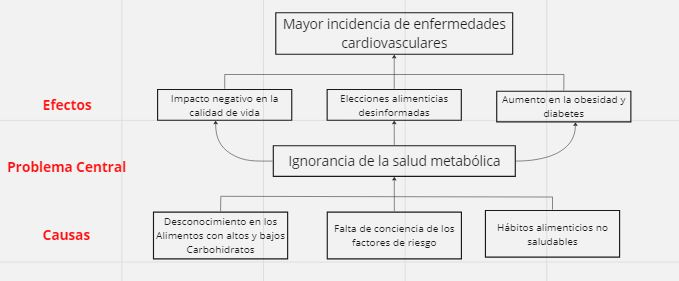
\includegraphics[width=1.1\textwidth]{1/figures/arbol de problems.JPG}
			\caption{Prueba de Figura}
			\label{fig1}
		\end{center}
		
	\end{figure}

\chapter{Anexo II: Árbol del objetivos}

\begin{figure}[h]
		\begin{center}
			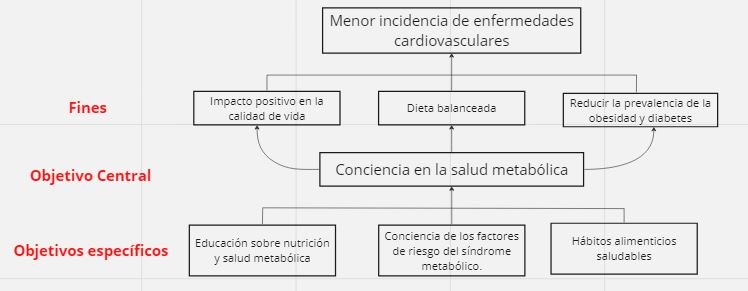
\includegraphics[width=1.1\textwidth]{1/figures/arbol de objetivos.JPG}
			\caption{Prueba de Figura}
			\label{fig1}
		\end{center}
		
	\end{figure}

\chapter{Anexo III: Matriz de Consistencia}

\begin{table}[h!]
	\centering
	\small
	\begin{tabular}{ |m{5cm}|m{5cm}|m{5cm}| }
		\hline
		\rowcolor{bluejean}
		\Centering \color{white}{PROBLEMAS}& \Centering \color{white}{OBJETIVOS}& \Centering \color{white}{HIPÓTESIS}\\
		\hline
		\rowcolor{turq}
		\Centering Problema General& \Centering Objetivo General & \Centering Hipotesis General \\
		\hline
  
        \ProblemaGeneral & 
        \ObjetivoGeneral  & 
        \HipotesisGeneral \\
        \hline
		
        \rowcolor{turq}
		\Centering Problemas Específicos& \Centering Objetivos Específicos & \Centering Hipotesis Específicas \\
		\hline
  
		{\Pbone} & {\Objone} & {\Hone} \\
		\hline
		{\Pbtwo} & {\Objtwo} & {\Htwo} \\
		\hline
		{\Pbthree} & {\Objthree} & {\Hthree} \\
		\hline
	\end{tabular}
	\caption{Matriz de consistencia. Fuente: Elaboración propia}
	\label{1:table}
\end{table}







% %%Bibliografia
%\bibliographystyle{apalike} % Title is link if provided
%\renewcommand{\bibname}{BIBLIOGRAFÍA} % changes the header; default: Bibliography

\printbibliography[heading=bibintoc,title={BIBLIOGRAFÍA}]
%\bibliography{biblio/references} % adjust this to fit your BibTex file
\end{document}

